% Evaluation
% Related with the requirements:
% Test 1: R1: pH Control: change constant's value and verify control work

\subsection{The Circuit Setup}

% \begin{figure}[h]
%     \centering
%     \includegraphics[width=.7\textwidth]{img/photo1.png}
%     \caption{A photo of the Water Cycle Control Circuit}
%     \label{fig:photo}
% \end{figure}

\subsection{A Graphical User Interface}

For the sake of making the unit tests to be shown in a written report,
a simple Graphical User Interface (GUI) has been implemented using Processing.
Processing is a simple programming language which is integrated with OpenGL,
Java and Serial communication.
So it is a reliable choice to display and transmit Serial data from/to Arduino within the computer screen.
But,
instead of being a monitoring-only GUI,
the Processing provides built-in functions to make mouse interactions easily,
hence the tests could be made faster.

\subsubsection{Simulation parameters}
\label{sec:simPar}

Concerning the pH variation during time,
a simple and rough approximation has been made, 
based on the expectation that the pH will vary lesser and lesser during time,
as the tank solution's pH becomes closer to the pH of the controlling pH tanks.

\subsubsection{A Simple Serial Communication Protocol}

To make the Arduino and Processing exchange messages and understand those exact meaning intended,
a simple protocol has been made allowing a simple handshake and several simple commands,
which can be interpreted as text messages.

\begin{table}[h]
\centering
\caption{Arduino--Processing Commands}
\label{tab:commands}
\begin{tabular}[h]{|l|l|l|}
    \hline
    \textbf{Command}     & \textbf{Source}    & \textbf{Meaning}
    \\\hline
    A           & Arduino    & Try to establish contact with a client
    \\\hline
    ACK         & Arduino    & Handshake is done
    \\\hline
    p<float>    & Processing & Send a hypothetical pH value of <float> \\ 
                &            & to simulate how the system responds to it
    \\\hline
    r           & Processing & Establish Contact or Retry Establishment
    \\\hline
\end{tabular}
\end{table}

The figure \ref{fig:sdProtocol} is a sequence diagram which describes in detail how the communication is made.
Note that the messages derived from $1$ are regarded to the connection phases,
and the messages derived from $2$ groups every command related to pH Control.

\begin{figure}[h]
    \centering
    \includegraphics[width=.5\textwidth]{diagrams/protocolSD.png}
    \caption{A sequence diagram depicting a connection between Arduino and Processing powered GUI followed by a pH Control request}
    \label{fig:sdProtocol}
\end{figure}

A screenshot of the serial monitor has been made to show a real example of the communication,
as follows in the figure \ref{fig:serialMonitor},
one can see that the pH of 7.5 was requested and the response is composed by 14 messages updating the pH value for each second,
with an extra one to finish the response packet and let Arduino to receive new pH values.
This relative high number of updates are expected,
since there the pH variation is simulated like as described in section \ref{sec:simPar}.

\begin{figure}[h]
    \centering
    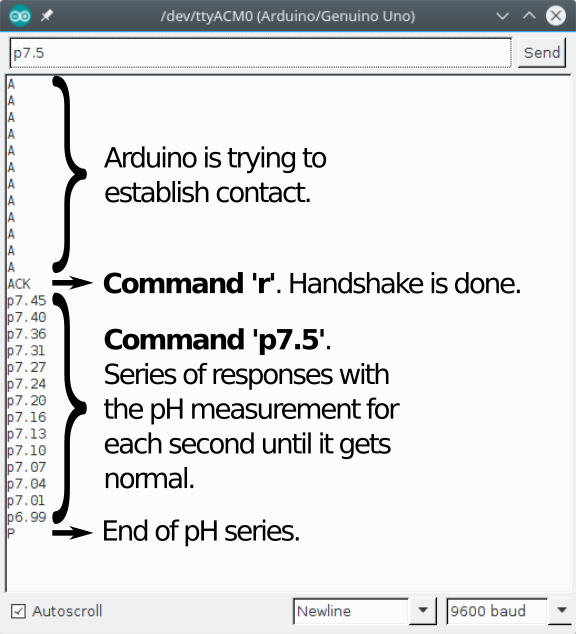
\includegraphics[width=.4\textwidth]{img/serialMon.png}
    \caption{The Arduino IDE Serial Monitor showing raw serial data}
    \label{fig:serialMonitor}
\end{figure}

\paragraph{Error Handling}

A classic retry connection option is available to make the interface more usable,
when the user has forgotten to connect the Arduino to the USB port,
for example.

\paragraph{IP Camera Support}
With the usage of the IP Capture library \cite{ipcapture_2016} and an Android App,
the author's camera turned into a IP Camera which can be displayed in real-time within the GUI.


\paragraph{A Video Overview}
\label{sec:video}


\begin{figure}[h]
    \centering
    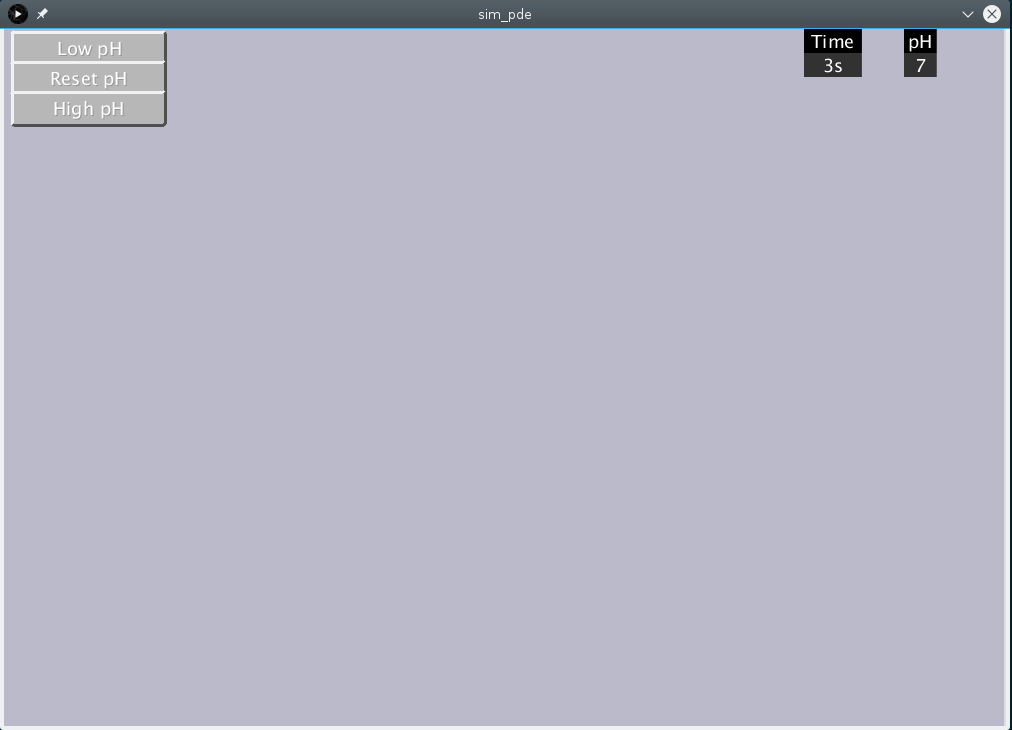
\includegraphics[width=.7\textwidth]{img/gui1.png}
    \caption{An initial version of the GUI}
    \label{fig:gui}
\end{figure}

\begin{figure}[h]
    \centering
    \includegraphics[width=.7\textwidth]{img/gui2.png}
    \caption{Using G4P plugin for Processing as the GUI library}
    \label{fig:g4p}
\end{figure}
